\documentclass[12pt,a4paper,portuguese]{article}

\usepackage[brazil]{babel}
\usepackage[utf8]{inputenc}
\usepackage[T1]{fontenc}
\usepackage[margin=1.5cm]{geometry}
\usepackage{multicol}
\usepackage{graphicx}
\usepackage{float}
\usepackage{subcaption}
\usepackage{enumerate}
\usepackage{listings}
\usepackage{xcolor}
\usepackage{amssymb}
\usepackage{amsmath}

\definecolor{gray}{HTML}{F2F2F2}
\definecolor{darkgray}{RGB}{77,77,77}
\definecolor{blue}{RGB}{53,53,104}
\definecolor{brown}{RGB}{139,88,88}

\lstset{
        basicstyle=\linespread{1.25}\small\ttfamily,
        showstringspaces=false,
        keywordstyle=\color{blue}\ttfamily,
        stringstyle=\color{brown}\ttfamily,
        commentstyle=\color{darkgray}\ttfamily,
        morecomment=[l][\color{blue}]{\#},
        backgroundcolor=\color{gray},
        breaklines=true,
        captionpos=b,
        caption=<avl.c>,
        numbers=left
    }

\begin{document}

    % Título
    \vspace{5mm}
    \rule{0.95\textwidth}{1pt}
    \vspace{3mm}
    \begin{center}
        \textbf{\huge Amigos de Graduação Indo ao Cinema} \\
        \Large Trabalho 2 \\
        \large SCC0223 Estruturas de Dados I
    
        \vspace{8mm}
        \begin{tabular}{rcl}
            Cody Stefano Barham Setti &-- &4856322 \\
            Luís Henrique de Queiroz Veras &-- &14592414 \\
            Raphael Mendes Batista &-- &15497660 \\
            Vinícius de Sá Ferreira &-- &15491650 \\
        \end{tabular}

    \vspace{8mm}
    08 de Dezembro de 2024
    \end{center}

    \vspace{1mm}
    \rule{0.95\textwidth}{1pt}
    \vspace{0.5cm}

    % Corpo do texto
    \section{Descrição do Trabalho Feito}
    \subsection{Visão Geral}
        Para desenvolver o sistema de cadastro de alunos de graduação e seus interesses cinematográficos, uma certa estrutura de dados foi fundamental: a árvore de Adelson-Velskii e Landis, ou, mais brevemente, a AVL.
        
        Duas instâncias de AVL foram utilizadas, uma árvore para armazenar os alunos cadastrados e outra para armazenar todos os filmes mencionados pelos alunos. A chave de ordenação utilizada na AVL de alunos foi o número USP. Os filmes, por sua vez, foram ordenados de forma alfabética. Portanto, o próprio nome de cada filme serve como sua respectiva chave.

        Por sua vez, os filmes favoritos de cada aluno individual foram armazenados em forma de lista ordenada (com cabeçalho). Entretanto, é importante frisar que os nós dessas listas foram reaproveitados da AVL de filmes -- para economizar memória -- logo, as listas, na realidade, são uma sequência estratégica de ponteiros.
        \begin{figure}[H]
            \centering
            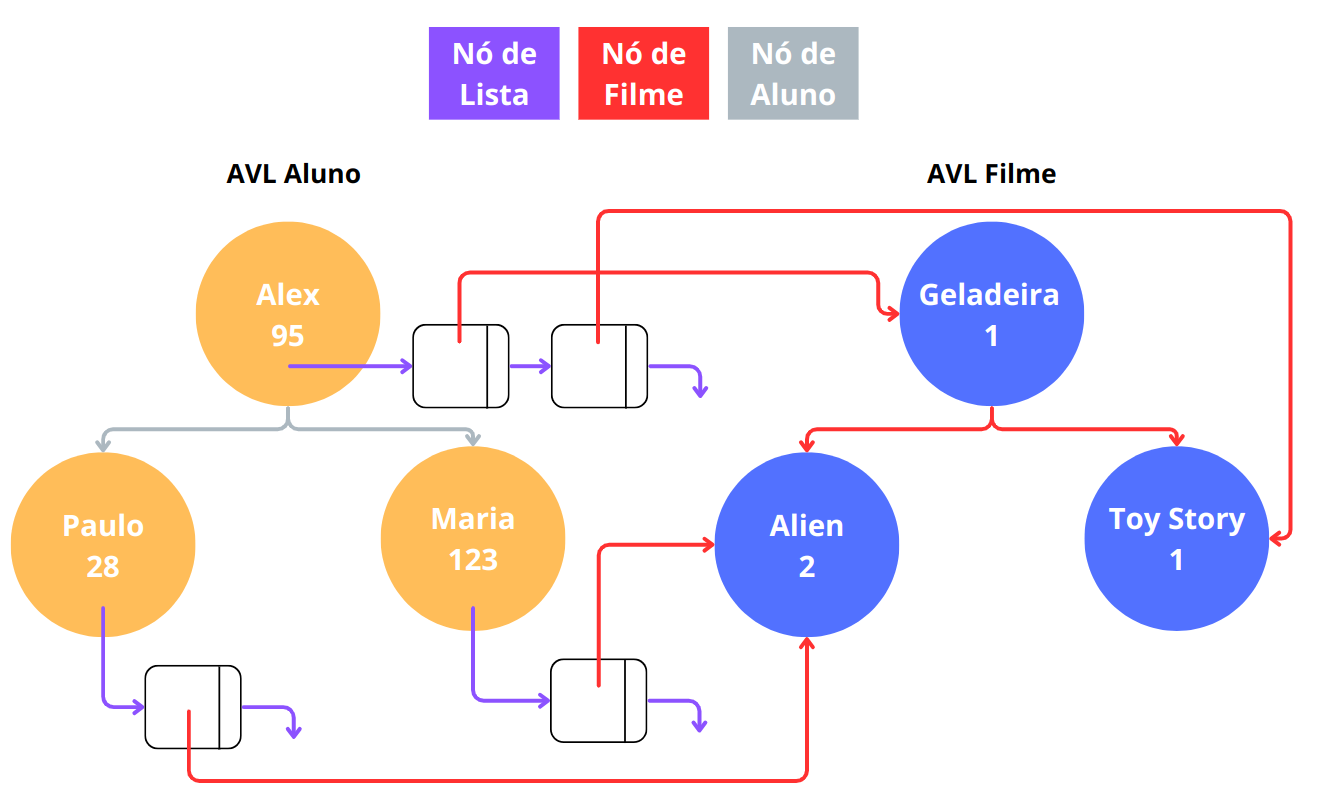
\includegraphics[height=8cm]{imgs/EsquemaED.png}
            \caption{Visão esquemática do armazenamento dos dados do trabalho}\label{fig:EsquemaEd}
        \end{figure}

        Finalmente, vale salientar que a estrutura de lista ordenada foi reaproveitada para a funcionalidade de impressão dos filmes mais queridos.

    \subsection{A Biblioteca `AVL'}
        Tratemos agora da implementação dessas estruturas basilares na linguagem de programação C, contida nos arquivos \verb|<avl.h>| e \verb|<avl.c>|.
    
    \subsubsection{Implementação da AVL}
        Primeiramente, ao se tratar da AVL, seus nós foram instanciados no tipo de dado \verb|no|. Tal dado faz uso de um \verb|enum|, para dá-lo a flexibilidade de armazenar as informações de um aluno ou de um filme. A \textit{flag} utilizada para indicar cada caso foi denominada de \verb|type|, onde \verb|type=0| indica o armazenamento do tipo \verb|aluno| e \verb|type=1| do tipo \verb|filme|.

        As variáveis armazenadas dentro desses dois tipos são
        \begin{itemize}
            \item[]\verb|aluno|:
            \begin{itemize}
                \item\verb|*nome|: um ponteiro do tipo \verb|char| para referenciar o primeiro caractere da \textit{string} que contém o nome do aluno.
                \item\verb|nroUSP|: uma variável do tipo \verb|int| para armazenar o número USP do respectivo aluno.
                \item\verb|*filmes_fav|: um ponteiro do tipo \verb|NoLista| (o qual será explicado posteriormente), para referenciar o cabeçalho da lista de filmes favoritos do aluno.
            \end{itemize}
            \item[]\verb|filme|:
            \begin{itemize}
                \item\verb|*nome|: um ponteiro do tipo \verb|char| para referenciar o primeiro caractere da \textit{string} que contém o nome do filme.
                \item\verb|frequencia|: uma variável do tipo \verb|int| que registra o número de alunos que adicionaram à sua lista de favoritos o respectivo \verb|filme|.
            \end{itemize}
        \end{itemize}
        O conjunto de \verb|type| com \verb|aluno|, ou então, com \verb|filme|, é amalgamado no tipo \verb|elem|. Por fim, além de seu \verb|elem|, todo \verb|no| possui também as variáveis
        \begin{itemize}
            \item[--]\verb|FB|: uma variável do tipo \verb|int|, utilizada para armazenar o fator de balanceamento do respectivo \verb|no| em relação à AVL à qual pertence.
            \item[--]\verb|altura|: uma variável do tipo \verb|int|, utilizada para armazenar a altura do respectivo \verb|no| em relação à AVL à qual pertence.
            \item[--]\verb|*esq|: um ponteiro a uma variável do tipo \verb|no|, que cumpre o papel de filho esquerdo na AVL.
            \item[--]\verb|*dir|: um ponteiro a uma variável do tipo \verb|no|, que cumpre o papel de filho direito na AVL.
        \end{itemize}

        Para as AVL's em si, criou-se o tipo de dado \verb|AVL|, que possui, simplesmente, um ponteiro \verb|*raiz|, que referencia o \verb|no| ocupando a raiz atual da árvore.

    \subsubsection{Implementação da Lista Ordenada}
        A instanciação dos nós das listas ordenadas ao invés de utilizar o tipo \verb|no|, aproveitou um tipo distinto, o \verb|NoLista|, que contém duas variáveis:
        \begin{itemize}
            \item[--]\verb|*filme|: um ponteiro para variáveis do tipo \verb|no|, a fim de referenciar itens da AVL de filmes.
            \item[--]\verb|*prox|: um ponteiro para variáveis do tipo \verb|NoLista|, para referenciar o próximo nó da lista ordenada.
        \end{itemize}
        O tipo \verb|Lista| foi definido para instanciar-se a lista, propriamente dita. De variáveis, ele contém simplesmente um ponteiro \verb|*ini|, que aponta ao seu primeiro \verb|NoLista|, o cabeçalho.

    \subsubsection{As Funções da Biblioteca `AVL'}
        Por fim, os arquivos \verb|<avl.h>| e \verb|<avl.c>| possuem algumas funções.
        
        Primeiro, há algumas correspondentes ao funcionamento elementar de uma AVL: \verb|Criar()| e \verb|FinalizarAVL()|, \verb|inserir()| e \verb|remover()|, que também rebalanceiam a árvore, e \verb|buscar()|, que aproveita a ordenação da árvore para fazer uma busca eficiente (tempo logarítmico) por um elemento na árvore.

        Ademais, para a conveniência do usuário, a biblioteca já inclui duas formas de imprimir os dados da AVL, encapsulados nas funções \verb|imprimirAVL()| e \verb|imprimirGrafo()|.
        \begin{figure}[H]
            \centering
            \begin{subfigure}[t]{0.3\textwidth}
                \centering
                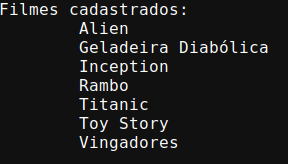
\includegraphics[height=3cm]{imgs/lista_filmes_LISTAS_3.png}
                \caption{\texttt{imprimirAVL()}}\label{fig:imprimirAVL}
            \end{subfigure}%
            \hfill
         \begin{subfigure}[t]{0.6\textwidth}
                \centering
                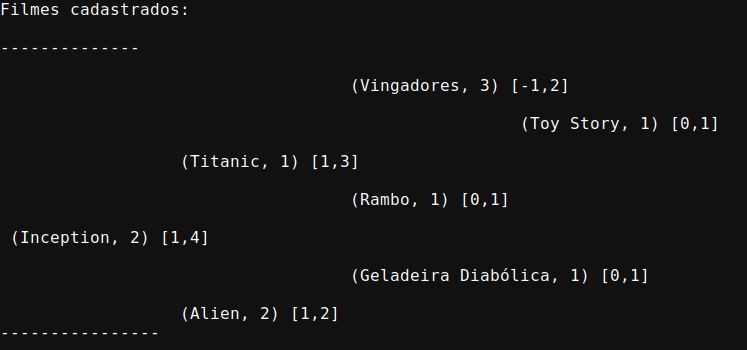
\includegraphics[height=5cm]{imgs/lista_filmes_ARVORE_3.png}
                \caption{\texttt{imprimirGrafo()}}\label{fig:imprimirGrafo}
            \end{subfigure}
            \caption{Os dois modos de imprimir as AVL's}
        \end{figure}

        Por fim, de interesse, há as funções \verb|imprimir_dadosAVL()| e \verb|salvar_sistema()|, que serão explicadas posteriormente, já que se referem diretamente a funcionalidades pedidas no projeto.

    \subsection{A Biblioteca `Aluno'}
        Os arquivos \verb|<aluno.h>| e \verb|<aluno.c>| encapsulam as funcionalidades específicas à AVL de alunos\footnote{Para seu funcionamento, é necessário a invocação da Biblioteca `AVL'.}.

        Nenhum tipo de dado novo é definido, apenas funções. Algumas, elementares, para a inserção e remoção de filmes da lista de favoritos de cada aluno. E outras mais elaboradas. Os dois algoritmos de sugestão de parceiros de cinema, \verb|sugerir_similar()| e \verb|sugerir_diferente()|; e uma função para suporte de edição de arquivos, \verb|carregar_arquivo()|.

    \subsection{A Biblioteca `Filme'}
        A biblioteca `Amigos de Graduação Indo ao Cinema' é completa com os arquivos \verb|<filme.h>| e \verb|<filme.c>|, cujo conteúdo resume-se à função \verb|mais_queridos()|, que lista o catálogo de filmes dos alunos em ordem de popularidade, mais suas funções auxiliares (escondidas do usuário).

    \subsection{Funcionalidades da Biblioteca}
        Conforme as especificações do trabalho, a biblioteca `Amigos de Graduação Indo ao Cinema' deve ser capaz de:
\begin{multicols}{2}
        \begin{enumerate}
            \item Cadastrar alunos em seu sistema;
            \item Remover de seu sistema o cadastro de um aluno;
            \item Dado um aluno, adicionar um filme à sua lista de prediletos;
            \item Dado um aluno, remover um filme de sua lista de prediletos;
            \item Listar todos os alunos cadastrados;
            \item Buscar um aluno específico no sistema;
            \item Listar os filmes cadastrados em ordem alfabética;
            \item Buscar um filme específico no sistema;
            \item Dado um aluno, indicá-lo um colega com gosto cinematográfico similar ao seu;
            \item Dado um aluno, indicá-lo um colega com gosto cinematográfico diferente ao seu;
            \item Salvar em um arquivo texto todas as informações armazenadas no sistema;
            \item Fornecer os dados técnicos das ABB's utilizadas: o número de nós de cada árvore, suas alturas totais e o maior fator de balanceamento dentre os nós das árvores;
            \item Listar os filmes em ordem de popularidade;
            \item Cadastrar alunos e seus filmes favoritos a partir de arquivo;
            \item Finalizar todos os dados;
            \item Limpar a tela;
            \item Modo de visualização. %
        \end{enumerate}
\end{multicols}
        Na função \verb|main()|, um menu é apresentado ao usuário, mostrando as 17 opções (mais a opção `0', para sair do sistema). Ele então digita qual quer utilizar e, internamente, um \verb|switch| faz o controle de quais funções da biblioteca chamar. Vejamos como cada funcionalidade foi implementada:
    \subsection*{Funcionalidade 1}
        O cadastro de alunos no sistema é feito pela função \verb|inserir()|, que, essencialmente, é um algoritmo de inserção de nós em uma AVL, ou seja, primeiro insere o aluno como uma folha, respeitando a estrutura de uma ABB, e, então, caso necessário, faz rotações para ajustar o balanceamento da árvore, a fim de que seja AVL.

        Utilizou-se a altura de cada nó para a checagem de balanceamento, assim há homogeneidade entre o funcionamento dos algoritmos de adição e remoção de alunos.
    \subsection*{Funcionalidade 2}
        Para cumprir tal funcionalidade primeiro é chamada a função \verb|limpar_filmes_fav()|, que remove da AVL de filmes aqueles cuja frequência torna-se 0, com a remoção do aluno em questão, e atualiza as frequências (subtrai 1) daqueles de sua lista ainda mencionados por outros alunos.

        Em seguida, a função \verb|remover()| é chamada, a qual remove da AVL de alunos o aluno em questão, certificando-se de rebalancear a árvore após.

    \subsection*{Funcionalidade 3}
        A função que, dado um aluno, adiciona um filme à sua lista de prediletos é a \verb|inserir_filme_fav()| da biblioteca `Aluno'.

        Ela opera de forma recursiva. Primeiramente, se o cabeçalho da lista de filmes favoritos não apresenta filmes na sequência, temos um caso base: o novo filme é inserido logo após o cabeçalho e retorna-se à função o valor \verb|1|, um \verb|int| que corresponde ao sucesso na inserção do filme na lista.
        
        Se esse não for o caso, vai-se percorrendo os nós da lista recursivamente até encontrar-se um cujo título de filme venha após, em ordem alfabética, o do novo que quer-se inserir na lista, indicado por um retorno de \verb|-1| (outro caso base).
        
        Com esse valor, a função sabe, então, que deve inserir o filme anteriormente a tal nó, para preservar-se a ordem alfabética e as chamadas anteriores de função todas retornam o valor \verb|1|.

        Caso todos os filmes da lista antecedam, em ordem alfabética, o filme novo que deseja-se inserir, a última vez que a função será chamada será para um nó \verb|NULL|. A função também tem retorno \verb|-1| neste caso e, portanto, ao voltar a penúltima chamada de função, insere o filme ao final da lista.

        Caso o usuário tente inserir um filme que já está na lista, na hora de compará-lo a si mesmo, não adentrará nenhum dos condicionais que checam se seu título vem estritamente antes ou após o do nó, retornando o valor \verb|0| (mais um caso base). As chamadas anteriores da função então também assumem tal valor e nada na lista é alterada.

        Por fim, caso haja erro de \verb|malloc|, a função retorna \verb|0|, pois nesse caso também não é possível inserir o filme na lista, já que falta espaço na memória para gravá-lo nela.

    \subsection*{Funcionalidade 4}
        Para a remoção de um filme predileto, está às ordens a função \verb|remover_filme_fav()|, cujo funcionamento é similar ao da função \verb|inserir_filme_fav()|, e a qual também pertence à biblioteca `Aluno'.

        A função é primeiro chamada para o cabeçalho da lista e, logo após, antes de cessar tal chamada, faz-se outra para o próximo nó. Se ele for nulo, a lista é inalterada e o chamado da função finalizado. Caso contrário, analisa-se se o filme de tal nó é o desejado para remoção. Se sim, o encadeamento da lista é rearranjado sem ele e ele é finalizado. Se não, prossegue-se ao próximo nó da lista.

        Ademais, na remoção, a frequência de aparição do filme no catálogo é diminuída. Se chegar a 0, no trecho de código da função \verb|main()| dedicado à funcionalidade 4, invoca-se a remoção do filme da AVL de filmes.
    \subsection*{Funcionalidade 5}
        A função que encarrega-se de listar todos os alunos cadastrados é a \verb|imprimirAVL()|, cujo funcionamento resume-se a chamar a função \verb|imprimir_recursivo()| para sua raiz.
        
        Tal função, por meio de uma recursão, percorre a árvore \textit{em ordem}: imprime a sub-árvore esquerda da raiz, depois a raiz e por fim sua sub-árvore direita. Consequentemente, os alunos são impressos em ordem crescente de número USP.

        Alternativamente, há a função \verb|imprimirGrafo()|, que invoca a função \verb|imprimir_recursivo2()|, para imprimir os dados em forma de árvore ao invés de lista. A alternância entre os dois modos de impressão é realizado na funcionalidade 17.

    \subsection*{Funcionalidade 6}
        A busca de um aluno específico no sistema é feita pela função \verb|buscar()|, a qual aproveita a ordenação da AVL: se a chave do elemento procurado for menor do que a do nó atual sendo analisado, procede-se ao seu filho esquerdo; caso contrário, o direito. Ou seja, \verb|buscar()| é uma função recursiva.

        Há algumas condições de parada: se a chave de um nó for a mesma daquela do aluno procurado, retorna-se o endereço de tal nó. Se chegar-se em um nó \verb|NULL|, o retorno da função é \verb|NULL|, para indicar que o aluno procurado não encontra-se na AVL.

    \subsection*{Funcionalidade 7}
        A listagem em ordem alfabética dos filmes cadastrados é feita novamente pela função \verb|imprimirAVL()|.
        
        Já que a árvore é de busca e o chaveamento da AVL de filmes é conforme seus nomes, a impressão \textit{em ordem} -- precisamente o modo adotado por \verb|imprimirAVL()| -- garante que os filmes sejam listados alfabeticamente.

    \subsection*{Funcionalidade 8}
        Como no caso da funcionalidade 6, a busca é feita por meio da função \verb|buscar()|, da biblioteca `AVL'.

    \subsection*{Funcionalidade 9}
        Primeiramente, é necessário explicar a métrica elegida para determinar o aluno de gosto mais similar ao colega em questão: o número de filmes em comum entre os dois. O último aluno encontrado na árvore (percorrida em ordem) de maior número de filmes em comum (excluindo o próprio colega), é elegido como aluno de gosto mais similar.

        Tal funcionalidade é encapsulada na função \verb|sugerir_similar()|. Por meio de uma recursão, ela percorre a AVL de alunos em ordem e, para cada nó, chama a subfunção \verb|filmes_fav_comum()|. Se \verb|filmes_fav_comum()| retornar um número maior ou igual do que o atual máximo, este é atualizado.

        Por sua vez, quanto ao funcionamento interno de \verb|filmes_fav_comum()|: aproveita-se de um \verb|while()| aliado ao fato das duas listas de filmes favoritos estarem em ordem alfabética para contar o número de filmes em comum: um índice \verb|i| é usado para percorrer a lista do colega, e outro \verb|j| para a lista do nó atual.
        \begin{itemize}
            \item Se o título do filme referente ao índice \verb|i| (filme na lista do colega) for menor do que o do indicado por \verb|j| (filme na lista do nó atual), faz-se um incremento em \verb|i|.

            \item Se for maior, faz-se um incremento em \verb|j|.

            \item Se forem iguais, faz-se um incremento em ambos \verb|i| e \verb|j|, e no número de filmes em comum.
        \end{itemize}
        O \verb|while| é finalizado quando ambos os índices tornam-se nulos, o que significa que todos filmes foram comparados.

    \subsection*{Funcionalidade 10}
        A métrica adotada neste caso é análoga ao do caso anterior, entretanto, elege-se o último aluno com o menor -- ao invés de maior -- número de filmes em comum com o colega.

        Tal funcionalidade é encapsulada na função \verb|sugerir_diferente()|, cuja única diferença em relação à função \verb|sugerir_similar()| é que o aluno a se sugerir é atualizado caso \verb|filmes_fav_comum()| encontrar outro com um número menor ou igual -- ao invés de maior ou igual -- de filmes em comum.

    \subsection*{Funcionalidade 11}
        Para salvar as informações do sistema em um arquivo \verb|.txt|, tem-se a função \verb|salvar_sistema()|. Ela cria ou sobrescreve o arquivo \verb|saida_sistema.txt|, pertencente ao diretório \verb|./src/|, conforme o seguinte padrão desenvolvido: percorrendo a AVL de alunos \textit{em ordem}, para cada nó seu, a função cria uma linha correspondente no arquivo e insere nela, na ordem apresentada, as seguintes informações,:
\begin{multicols}{3}
        \begin{enumerate}
            \item Nome do aluno;
            \item Número USP do aluno;
            \item Nome dos filmes favoritos.
        \end{enumerate}
\end{multicols}
        Utiliza-se o ponto e vírgula como separados dessas informações.
    \subsection*{Funcionalidade 12}
        Os três dados técnicos sobre as ABB's utilizadas são fornecidos conjuntamente pela função \\\verb|imprimir_dadosAVL()|, que invoca três sub-rotinas:
        \begin{enumerate}
            \item\verb|numero_nos()|: Uma função recursiva que percorre a árvore em pré-ordem, dando um incremento unitário ao seu contador de nós\footnote{O próprio retorno da função.} a cada recursão. Seu passo base é quando depara-se com um nó \verb|NULL|. Neste caso, retorna 0.
            
            \item\verb|altura()|: Já que a altura de cada nó deve ser monitorada para o balanceamento da AVL, a função \verb|altura()| aproveita-se desse fato e simplesmente recupera a altura de sua raiz.
            
            \item\verb|maior_FB()|: O fato de optarmos pelo uso de AVL traz um de seus maiores facilitadores aqui. Pela teoria de AVL, sabe-se que, se houver uma diferença de altura entre suas sub-árvores, ela terá módulo igual a 1, pois diferenças maiores não são admitidas. Se não houver diferenças de altura, isso implica que o FB de todos seus nós será 0.
            
            Consequentemente, \verb|maior_FB()| simplesmente percorre a AVL em \textit{pré-ordem} e, se encontrar um nó com $\lvert\operatorname{FB}\rvert=1$, cessa a busca, retornando 1. Caso percorra a árvore inteira sem adentrar o condicional, retorna 0.
        \end{enumerate}

    \subsection*{Funcionalidade 13}
        A listagem dos filmes em ordem de popularidade é encapsulada na função \verb|mais_queridos()|. A função começa criando tal lista. Caso haja espaço na memória para tanto, prossegue para inserção dos filmes nela, feita pela função auxiliar \verb|inserirListaFreq()|.

        Por sua vez, \verb|inserirListaFreq()| percorre a AVL de filmes \textit{em ordem} e, para a ordenação, faz uso da função \verb|inserir_recursivo()|.

        Finalmente, \verb|inserir_recursivo()|, dada a lista de filmes populares em formação e um nó da AVL de filmes, checa a popularidade do nó em relação aos elementos da lista, inserindo-o após os de popularidade estritamente maior (os detalhes são análogos ao funcionamento da função \verb|inserir_filme_fav()|, pois, em ambos os casos, está-se reordenando uma lista após a inserção de um elemento novo).

        Vale salientar que os filmes de mesma popularidade estarão listados em ordem alfabética, pois a AVL de filmes foi percorrida \textit{em ordem}, como também sempre insere-se filmes de frequência 1 ao fim da lista, tanto para preservar esse `sub-ordenamento', como para fins de otimização.

    \subsection*{Funcionalidade 14}
        O cadastro de alunos e seus respectivos filmes favoritos no sistema a partir de um arquivo \verb|.txt| é feito por meio da função \verb|carregar_arquivo()|.

        Arquivos para leitura, igualmente aos para salvar o sistema, são mantidos no diretório \verb|./src/|. Entretanto, apenas um foi desenvolvido: \verb|entrada_sistema.txt|. Sua formatação segue a mesma lógica do arquivo \verb|salvar_sistema.txt|: cada linha é dedicada a um aluno, cujos dados são separados pelo ponto e vírgula e, presume-se que sua ordem seja
\begin{multicols}{3}
        \begin{enumerate}
            \item Nome do aluno;
            \item Número USP;
            \item Nome dos filmes favoritos.
        \end{enumerate}
\end{multicols}
        Não é necessário fornecer informações completas. Entretanto, alguns casos podem acusar erros, como, por exemplo, fornecer o nome de um aluno sem número USP.

        São feitas checagens: se o aluno já encontra-se no sistema (acusa um erro nesse caso), e se filmes favoritos foram repetidos, para que as listas dos alunos não contenham redundância, nem haja erro na popularidade do catálogo.

    \subsection*{Funcionalidade 15}
        A finalização de todos os dados é feita chamando-se a função \verb|FinalizarAVL()| duas vezes. Uma para a árvore de alunos, e outra para a de filmes.

        Tal função percorre as árvores de forma \textit{pós-ordem}. Caso contrário, a referência a sub-árvores seria perdida ao deletar-se a raiz primeiro.

        Para o caso da AVL de alunos, uma função auxiliar \verb|finalizarLista()| é invocada antes de deletar-se o respectivo nó, a fim de finalizar também a lista de filmes favoritos do aluno correspondente. Isso é feito percorrendo-se a lista de filmes favoritos até seu fim e, então, voltando e deletando seus nós no caminho, o que inclui o cabeçalho da lista.

        Para a AVL de filmes, a função \verb|FinalizarAVL()| imediatamente finalizar os nós, já que não há listas atrelados a eles.

        Por fim, salienta-se que depois dessas chamadas de funções, resta uma raiz para cada AVL. Entretanto, no arquivo \verb|main.c|, em que a funcionalidade 15 está implementada, as AVL's são definitivamente finalizadas.

    \subsection*{Funcionalidade 16}
        Simplesmente, a tela do terminal é limpada por meio do comando nativo \verb|system("clear")| para a implementação em LINUX, ou então o comando \verb|system("cls")| para a em Windows, visando a qualidade de vida do usuário.

    \subsection*{Funcionalidade 17}
        Desenvolveu-se um modo de visualização alternativa para os dados das AVL's. No lugar de listar os alunos ou filmes, são mostrados conforme seu armazenamento nas árvores.

        Logo, a funcionalidade 17 permite ao usuário alternar entre o modo de visualização em lista e o em árvore, este segundo internamente denominado de \verb|impressaoGrafo()|.

    \section{Estruturas de Dados Utilizadas e Justificativas}
        As estruturas de dados utilizadas foram AVL e lista dinâmica encadeada ordenada com cabeçalho.

        A estrutura de AVL foi utilizada por dois motivos. Primeiro, ela é excelente para receber e armazenar ordenadamente dados fornecidos de forma aleatória. Segundo, o fato dela preservar um balanceamento sempre, garante que o custo temporal de percorrê-la sempre seja bem próximo de $O(\log(n))$, onde $n$ é o número de nós na árvore.

        Por sua vez, já que cada aluno deve ter uma respectiva lista de filmes favoritos, ordenados de forma alfabética, utilizou-se uma lista com cabeçalho, pois o cabeçalho facilita a implementação de algoritmos de ordenação.

    \setcounter{section}{2}
    \section{Apresentação do Sistema}
        \subsection{Compilador Utilizado}

        \begin{figure}[H]
            \centering
            
\includegraphics[height=4cm]{imgs/versao_compilador.png}
        \end{figure}

        \subsection{Rodagem do Programa}

        \begin{figure}[H]
            \centering
            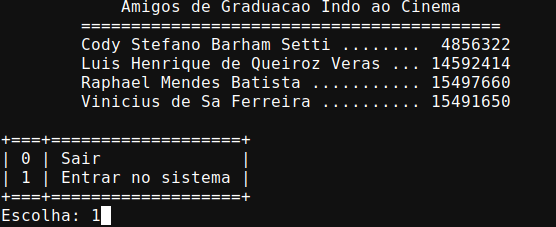
\includegraphics[height=5cm]{imgs/menu_inicial.png}
            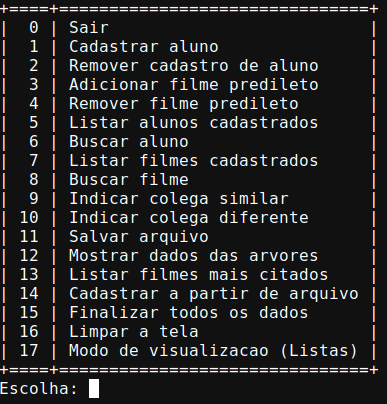
\includegraphics[height=5cm]{imgs/menu_funcoes.png}
            \caption{Menus}
        \end{figure}

        \begin{figure}[H]
            \centering
            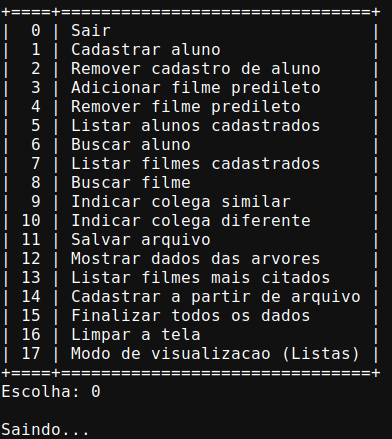
\includegraphics[height=5cm]{imgs/sair.png}
            \caption{Sair}
        \end{figure}

        \begin{figure}[H]
            \centering
            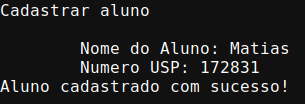
\includegraphics[height=1.5cm]{imgs/cadastra_aluno_1.png}
            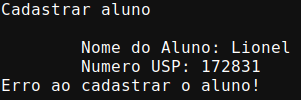
\includegraphics[height=1.5cm]{imgs/cadastra_aluno_2.png}
            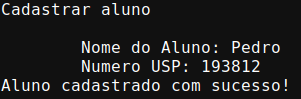
\includegraphics[height=1.5cm]{imgs/cadastra_aluno_3.png}
            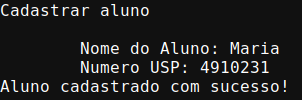
\includegraphics[height=1.5cm]{imgs/cadastra_aluno_4.png}
            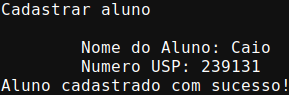
\includegraphics[height=1.5cm]{imgs/cadastra_aluno_5.png}
            \caption{Cadastro de alunos}
        \end{figure}

        \begin{figure}[H]
            \centering
            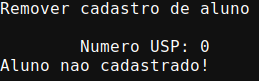
\includegraphics[height=1.5cm]{imgs/remove_cadastro_1.png}
            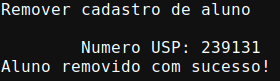
\includegraphics[height=1.5cm]{imgs/remove_cadastro_2.png}
            \caption{Remove cadastro de aluno}
        \end{figure}

        \begin{figure}[H]
            \centering
            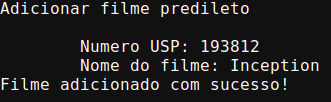
\includegraphics[height=1.5cm]{imgs/adiciona_filme_1.png}
            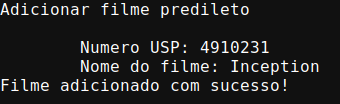
\includegraphics[height=1.5cm]{imgs/adiciona_filme_2.png}
            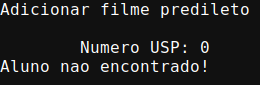
\includegraphics[height=1.5cm]{imgs/adiciona_filme_3.png}
            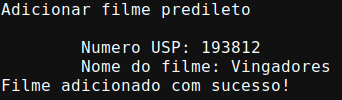
\includegraphics[height=1.5cm]{imgs/adiciona_filme_4.png}
            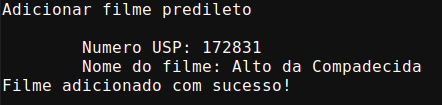
\includegraphics[height=1.5cm]{imgs/adiciona_filme_5.png}
            \caption{Adiciona os filmes prediletos dos alunos}
        \end{figure}

        \begin{figure}[H]
            \centering
            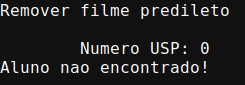
\includegraphics[height=1.5cm]{imgs/remove_filme_1.png}
            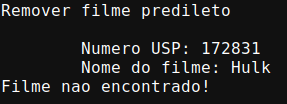
\includegraphics[height=1.5cm]{imgs/remove_filme_2.png}
            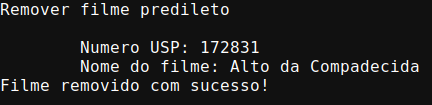
\includegraphics[height=1.5cm]{imgs/remove_filme_3.png}
            \caption{Remove os filmes prediletos dos alunos}
        \end{figure}

        \begin{figure}[H]
            \centering
            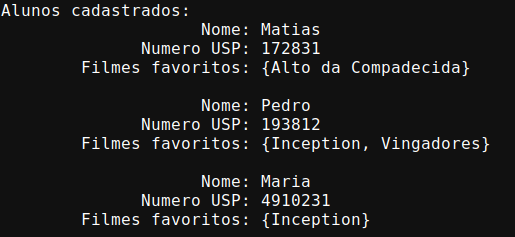
\includegraphics[height=3cm]{imgs/lista_alunos_LISTAS_1.png}
            \vspace{-10px}
            \caption*{Figura 9.1: Antes da remoção do filme predileto de Matias}
            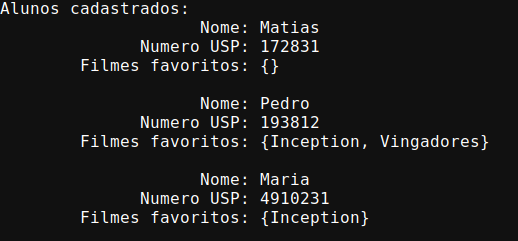
\includegraphics[height=2.95cm]{imgs/lista_alunos_LISTAS_2.png}
            \vspace{-10px}
            \caption*{Figura 9.2: Depois da remoção do filme predileto de Matias}
            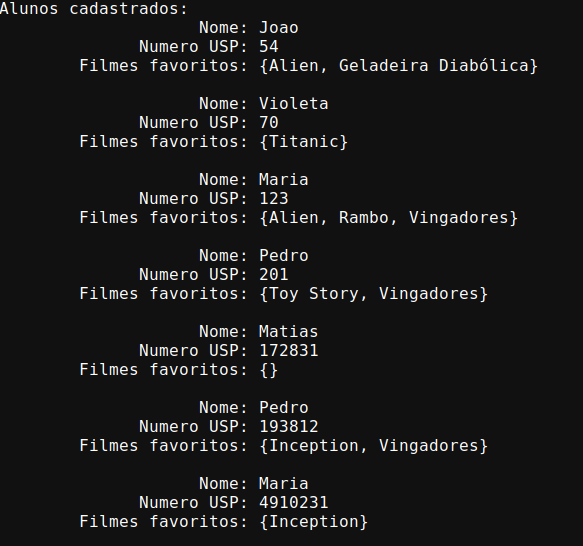
\includegraphics[height=6.8cm]{imgs/lista_alunos_LISTAS_3.png}
            \vspace{-10px}
            \caption*{Figura 9.3: Depois de carregar os dados de arquivo}
            Figura 9: Lista alunos cadastrados, no modo de visualização \texttt{Listas}
        \end{figure}

        \setcounter{figure}{9}

        \begin{figure}[H]
            \centering
            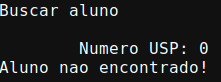
\includegraphics[height=2.8cm]{imgs/busca_aluno_1.png}
            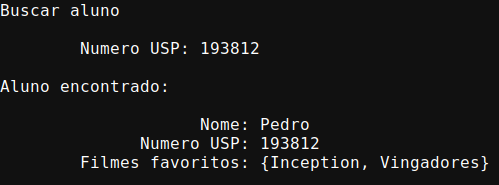
\includegraphics[height=2.8cm]{imgs/busca_aluno_2.png}
            \caption{Busca alunos}
        \end{figure}

        \begin{figure}[H]
            \centering
            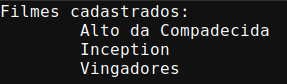
\includegraphics[height=2cm]{imgs/lista_filmes_LISTAS_1.png}
            \vspace{-10px}
            \caption*{Figura 11.1: Antes da remoção do filme predileto de Matias}
            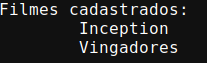
\includegraphics[height=2cm]{imgs/lista_filmes_LISTAS_2.png}
            \vspace{-10px}
            \caption*{Figura 11.2: Depois da remoção do filme predileto de Matias}
            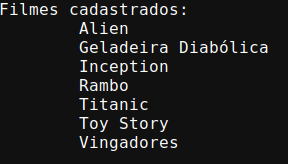
\includegraphics[height=4cm]{imgs/lista_filmes_LISTAS_3.png}
            \vspace{-10px}
            \caption*{Figura 11.3: Depois de carregar os dados de arquivo}
            Figura 11: Lista alunos cadastrados, no modo de visualização \texttt{Listas}
        \end{figure}

        \setcounter{figure}{11}

        \begin{figure}[H]
            \centering
            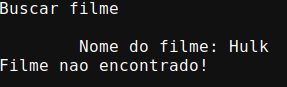
\includegraphics[height=2.1cm]{imgs/busca_filme_1.png}
            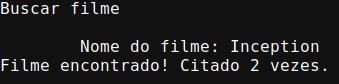
\includegraphics[height=2.1cm]{imgs/busca_filme_2.png}
            \caption{Busca filmes}
        \end{figure}

        \begin{figure}[H]
            \centering
            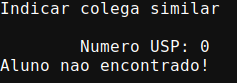
\includegraphics[height=1.5cm]{imgs/indica_similar_1.png}
            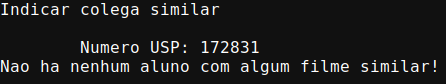
\includegraphics[height=1.5cm]{imgs/indica_similar_2.png}
            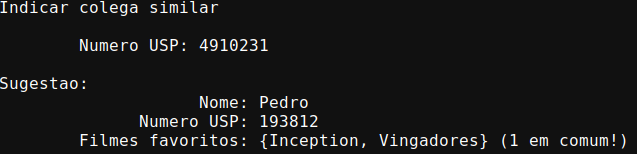
\includegraphics[height=2.7cm]{imgs/indica_similar_3.png}
            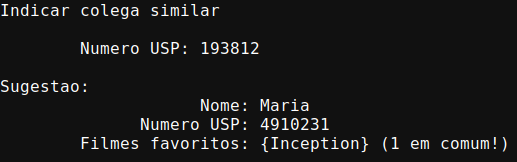
\includegraphics[height=2.7cm]{imgs/indica_similar_4.png}
            \caption{Indica um colega que tenha filmes similares}
        \end{figure}

        \begin{figure}[H]
            \centering
            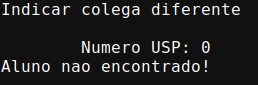
\includegraphics[height=1.5cm]{imgs/indica_diferente_1.png}
            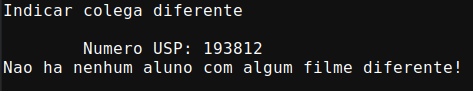
\includegraphics[height=1.5cm]{imgs/indica_diferente_3.png}
            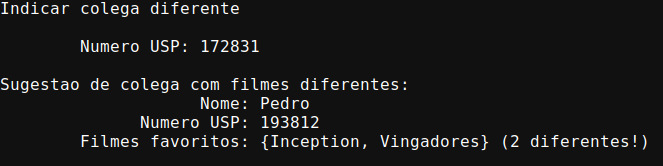
\includegraphics[height=2.7cm]{imgs/indica_diferente_2.png}
            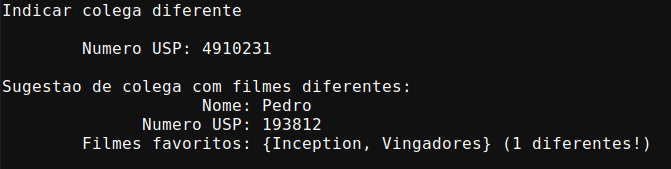
\includegraphics[height=2.7cm]{imgs/indica_diferente_4.png}
            \caption{Indica um colega que tenha filmes diferentes}
        \end{figure}

        \begin{figure}[H]
            \centering
            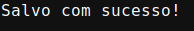
\includegraphics[height=1.5cm]{imgs/salva_sistema.png}
            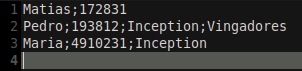
\includegraphics[height=1.5cm]{imgs/salva_sistema_gerado.png}
            \caption{Salva os dados no arquivo \texttt{src/saida\_sistema.txt}}
        \end{figure}

        \begin{figure}[H]
            \centering
            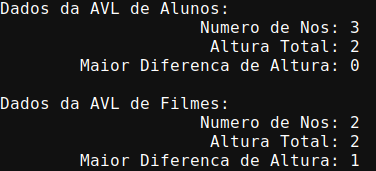
\includegraphics[height=3cm]{imgs/mostra_dados_arvores.png}
            \vspace{-10px}
            \caption*{Figura 16.1: Antes de carregar os dados de arquivo}
            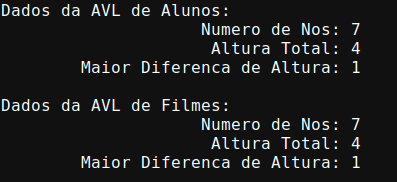
\includegraphics[height=3cm]{imgs/mostra_dados_arvores_2.png}
            \vspace{-10px}
            \caption*{Figura 16.2: Depois de carregar os dados de arquivo}
            Figura 16: Mostra os dados da AVL de alunos e da AVL de filmes
        \end{figure}

        \begin{figure}[H]
            \centering
            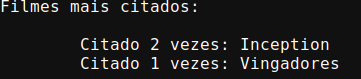
\includegraphics[height=2cm]{imgs/filmes_mais_citados.png}
            \vspace{-10px}
            \caption*{Figura 17.1: Antes de carregar os dados de arquivo}
            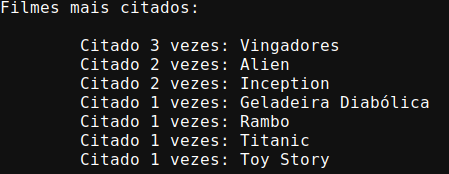
\includegraphics[height=3.6cm]{imgs/filmes_mais_citados_2.png}
            \vspace{-10px}
            \caption*{Figura 17.2: Depois de carregar os dados de arquivo}
            Figura 17: Mostra os filmes mais citados em ordem decrescente
        \end{figure}

        \setcounter{figure}{17}

        \begin{figure}[H]
            \centering
            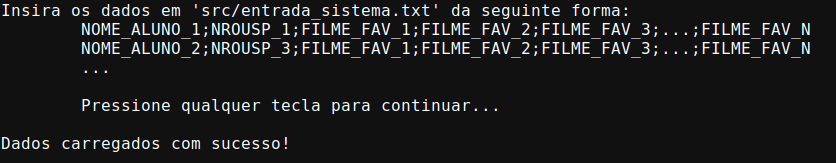
\includegraphics[height=3cm]{imgs/carregar_de_arquivo.png}
            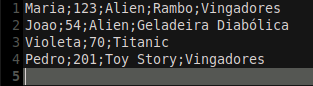
\includegraphics[height=2cm]{imgs/carregar_de_arquivo_insercao.png}
            \caption{Lê os dados do arquivo \texttt{src/entrada\_sistema.txt}}
        \end{figure}

        \begin{figure}[H]
            \centering
            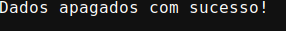
\includegraphics[height=.6cm]{imgs/finaliza_todos_os_dados.png}
            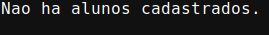
\includegraphics[height=.6cm]{imgs/lista_alunos_finalizado.png}
            \includegraphics[height=.6cm]{imgs/lista_filmes_finalizado.png}
            \includegraphics[height=1.5cm]{imgs/mostra_dados_arvores_finalizado.png}
            \includegraphics[height=1.5cm]{imgs/filmes_mais_citados_finalizado.png}
            \caption{Finaliza todos os dados das duas AVL's}
        \end{figure}

        \begin{figure}[H]
            \centering
            \includegraphics[width=6cm]{imgs/modo_de_visualizacao_1.png}\\
            \includegraphics[height=3.8cm]{imgs/lista_alunos_ARVORE_1.png}
            \includegraphics[height=3.8cm]{imgs/lista_filmes_ARVORE_1.png}
            \vspace{-10px}
            \caption*{Figura 20.1: Antes de carregar os dados de arquivo e antes da remoção do filme predileto de Matias}
            \includegraphics[width=8cm]{imgs/lista_filmes_ARVORE_2.png}
            \vspace{-10px}
            \caption*{Figura 20.2: Antes de carregar os dados de arquivo e depois da remoção do filme predileto de Matias}
            \includegraphics[height=4.2cm]{imgs/lista_alunos_ARVORE_2.png}
            \includegraphics[height=4.2cm]{imgs/lista_filmes_ARVORE_3.png}
            \vspace{-10px}
            \caption*{Figura 20.3: Depois de carregar os dados de arquivo}
            Figura 20: Alterna o modo de visualização de \texttt{Listas} para \texttt{Arvore}
        \end{figure}
\end{document}